\sect{Ćwiczenia 2}

\begin{frame}{Zadanie 1}
	\begin{figure}
		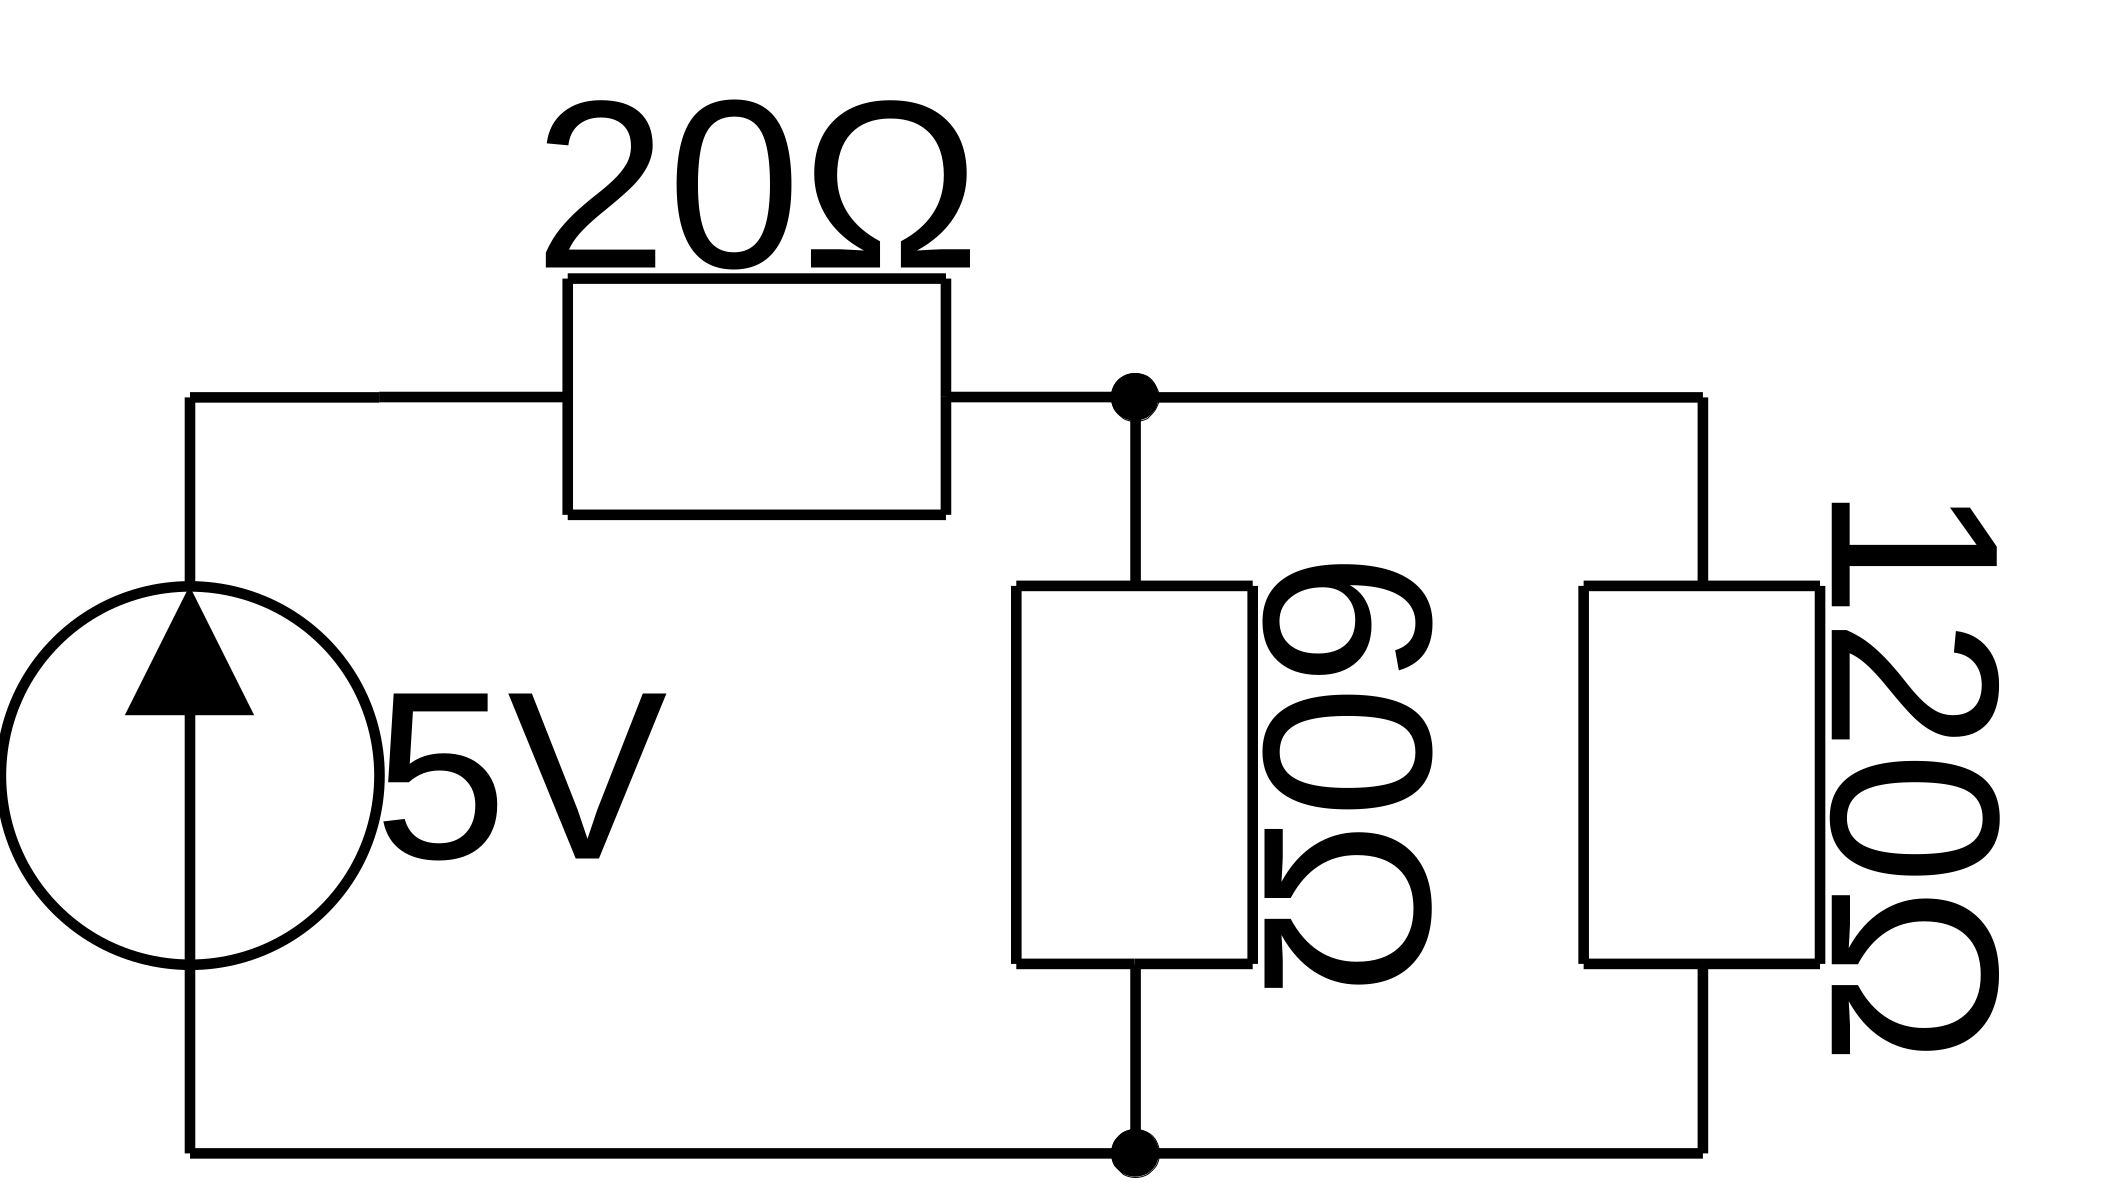
\includegraphics[scale=0.12, alt={}]{./imags/E02/2a.png}
		\caption{Zadanie 1. Oblicz wszystkie napięcia i prądy.}
	\end{figure}	
\end{frame}

\begin{frame}{Zadanie 2}
	\begin{figure}
		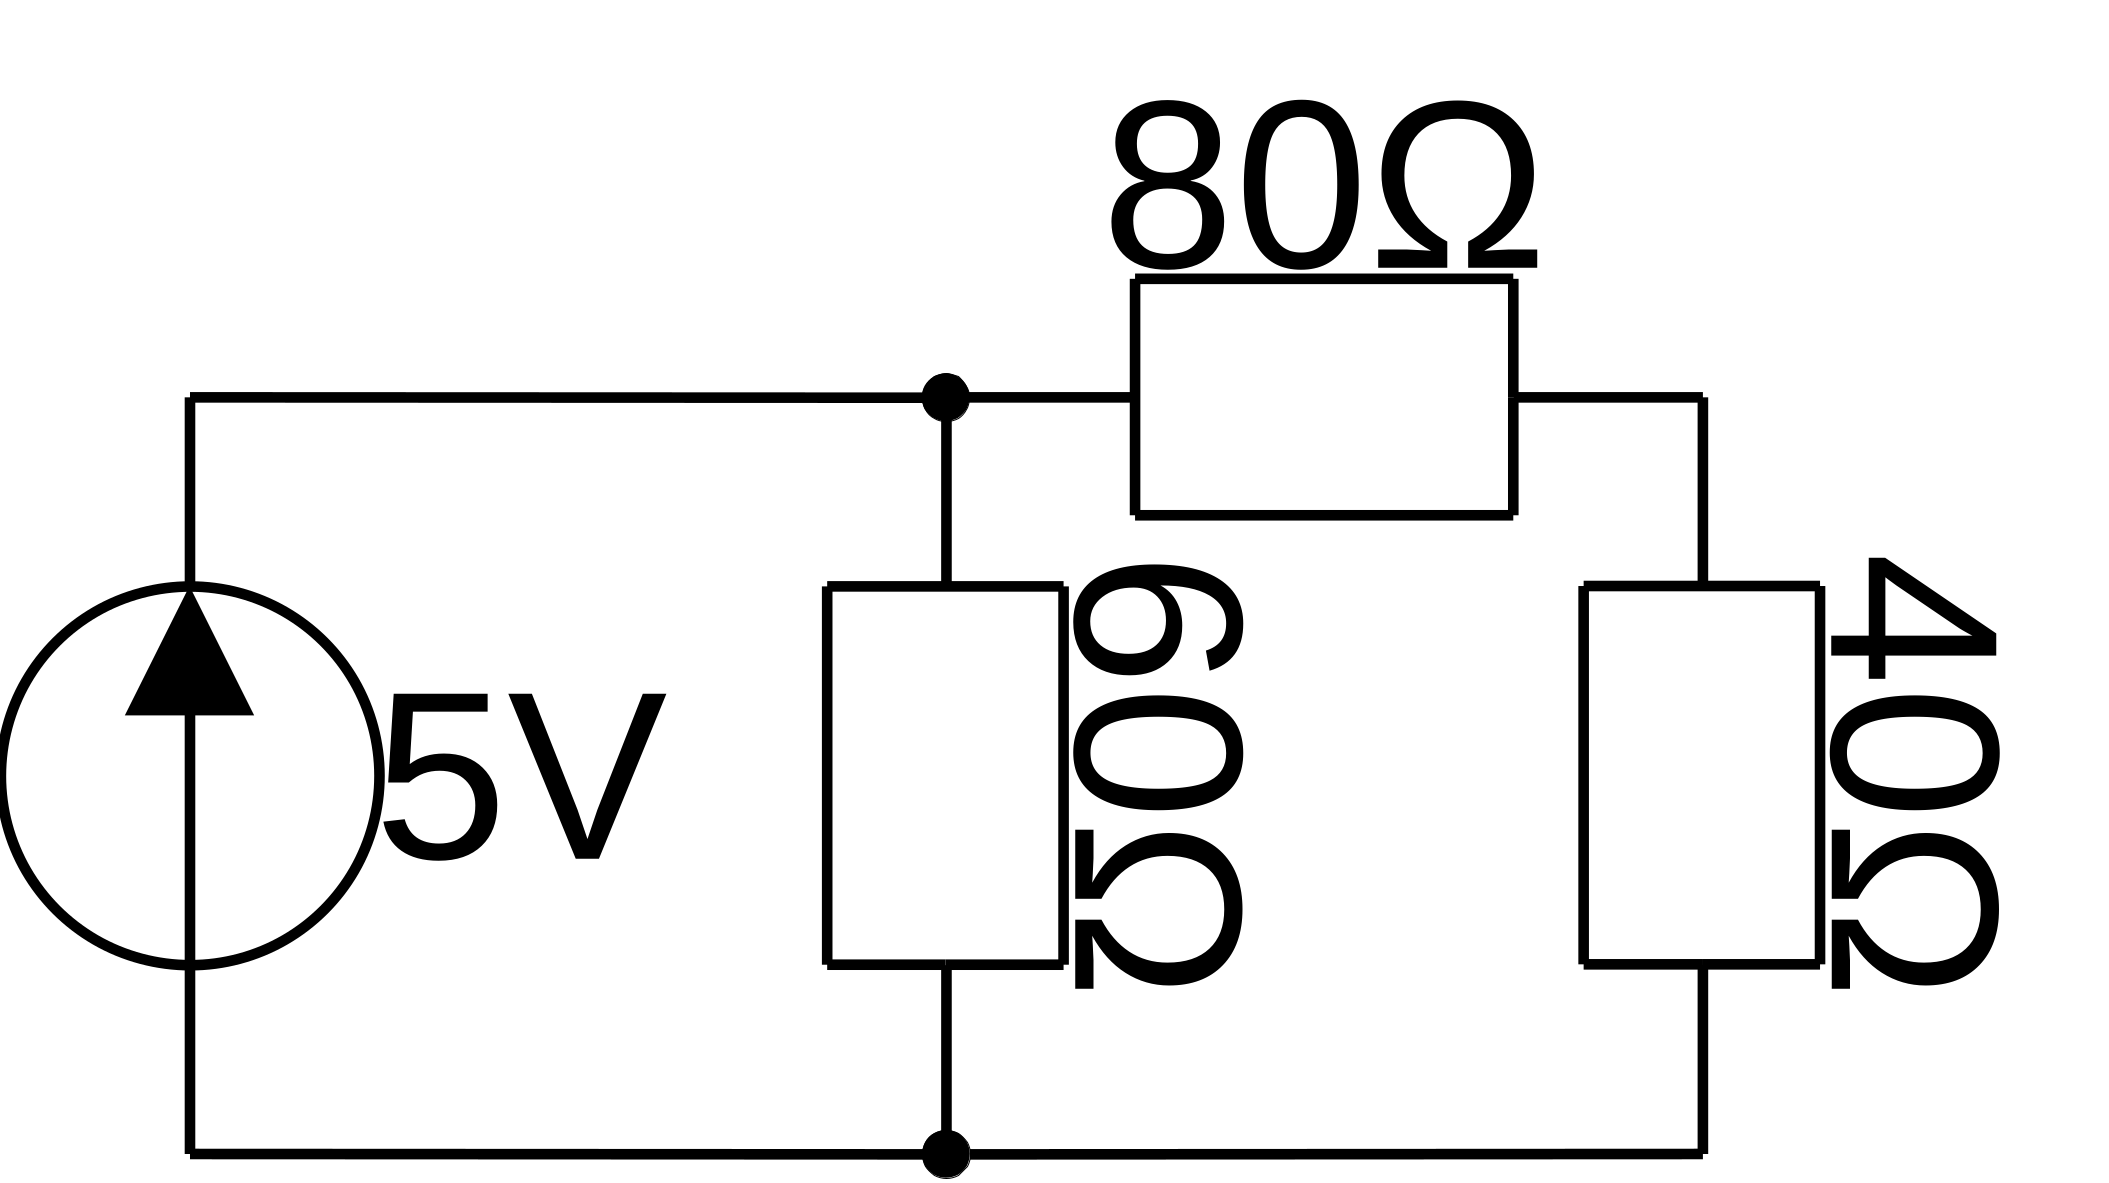
\includegraphics[scale=0.12, alt={}]{./imags/E02/2b.png}
		\caption{Zadanie 2. Oblicz wszystkie napięcia i prądy.}
	\end{figure}	
\end{frame}

\begin{frame}{Zadanie 3}
	\begin{figure}
		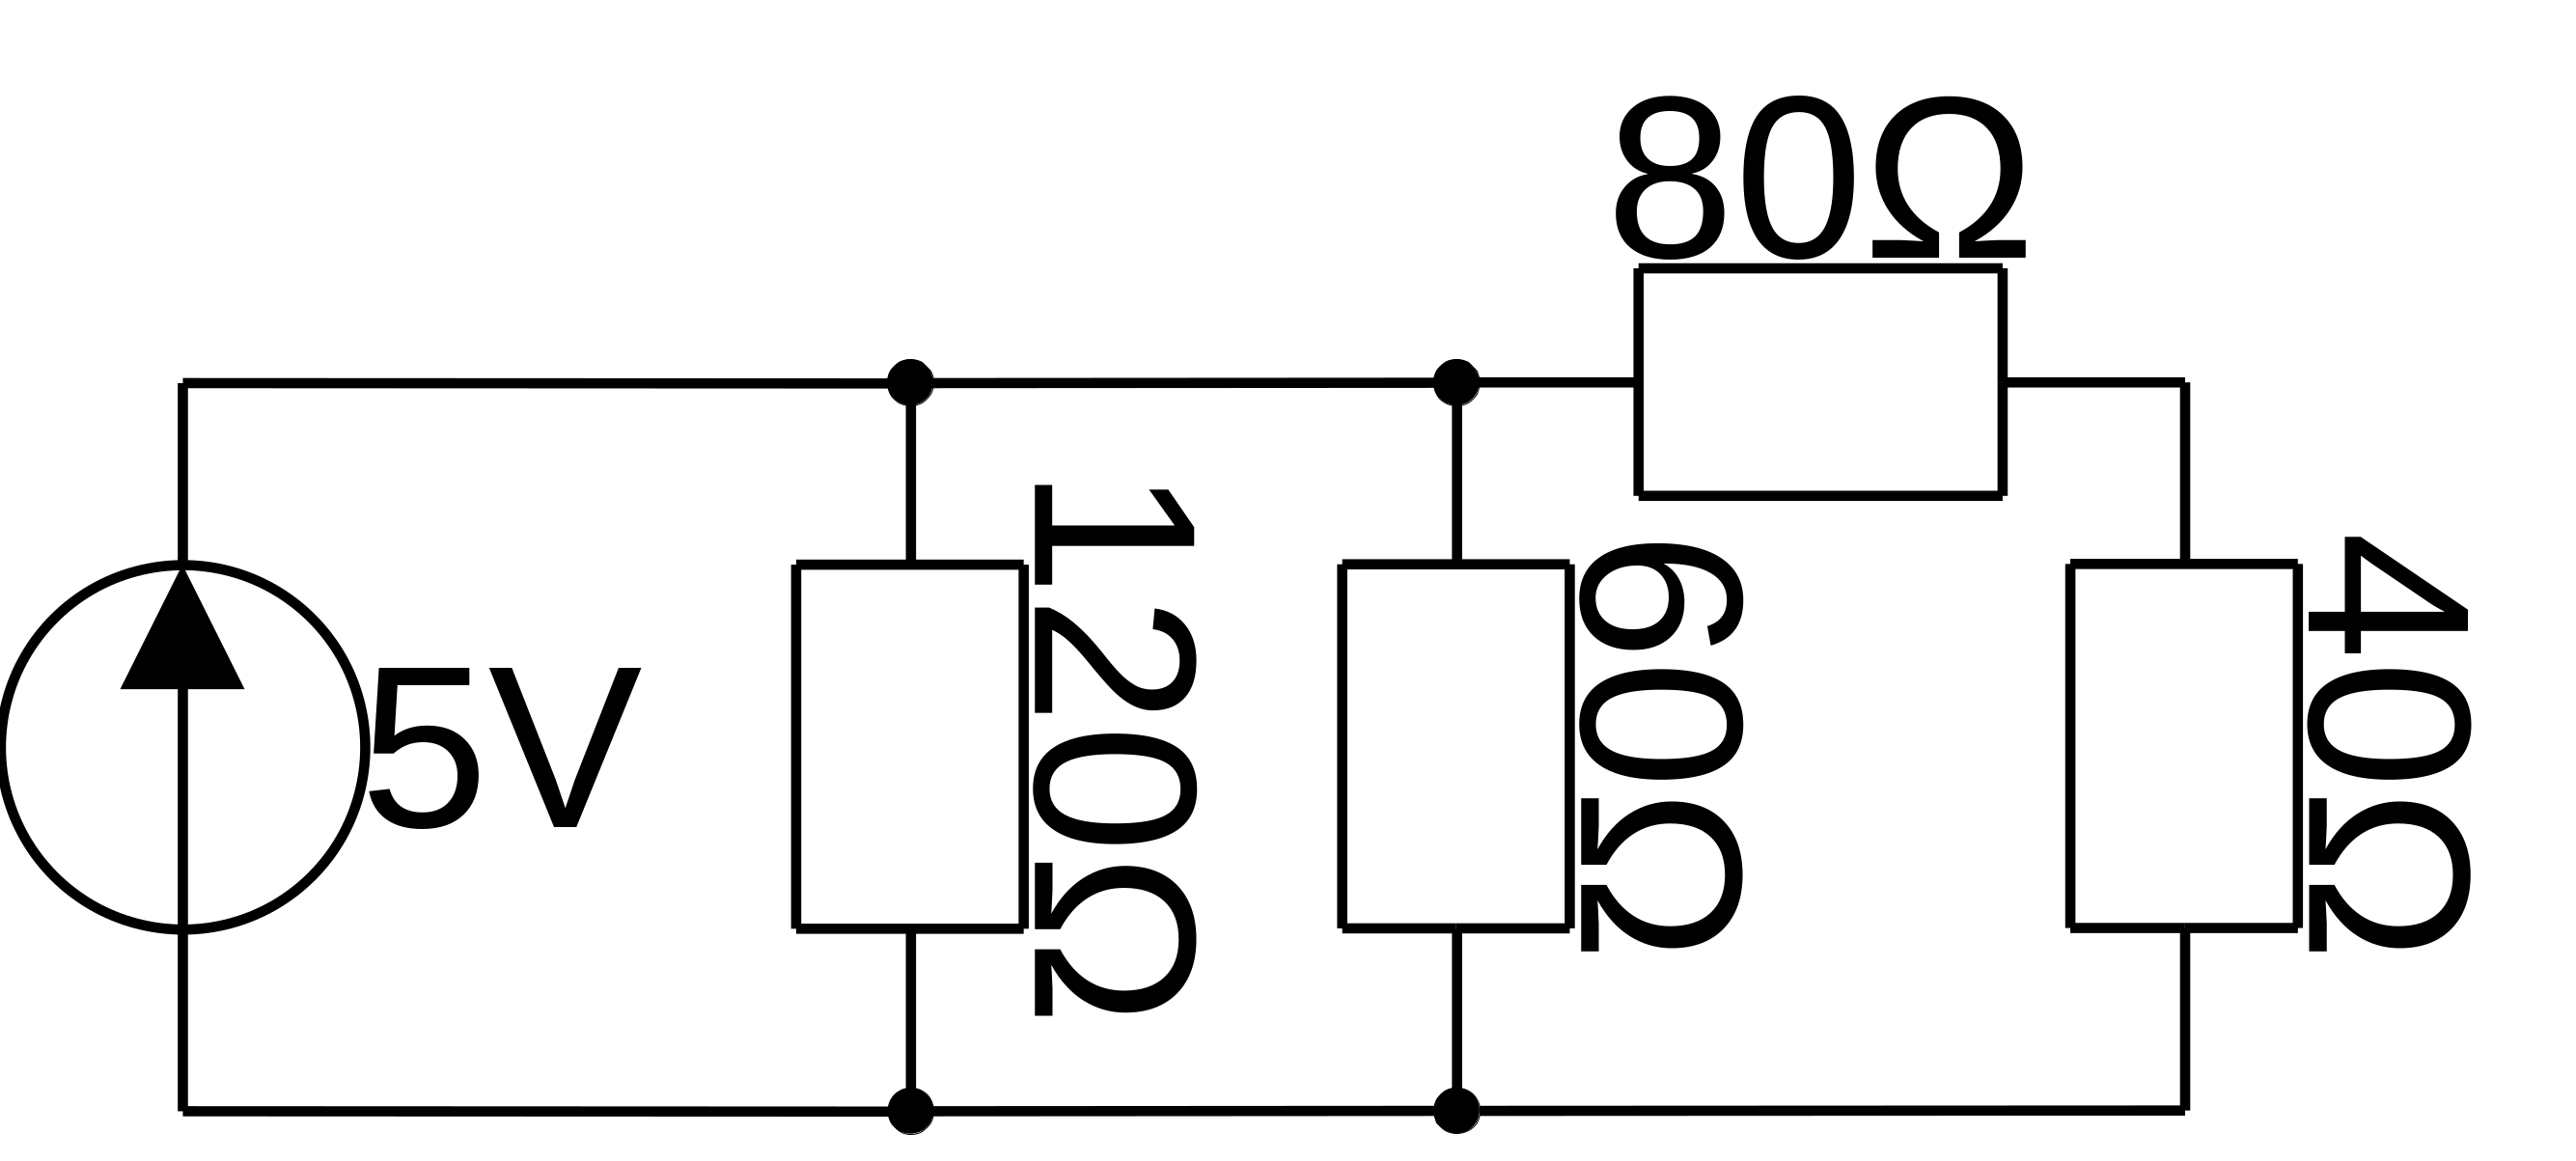
\includegraphics[scale=0.12, alt={}]{./imags/E02/2c.png}
		\caption{Zadanie 3. Oblicz wszystkie napięcia i prądy.}
	\end{figure}	
\end{frame}

\begin{frame}{Zadanie 4}
	\begin{figure}
		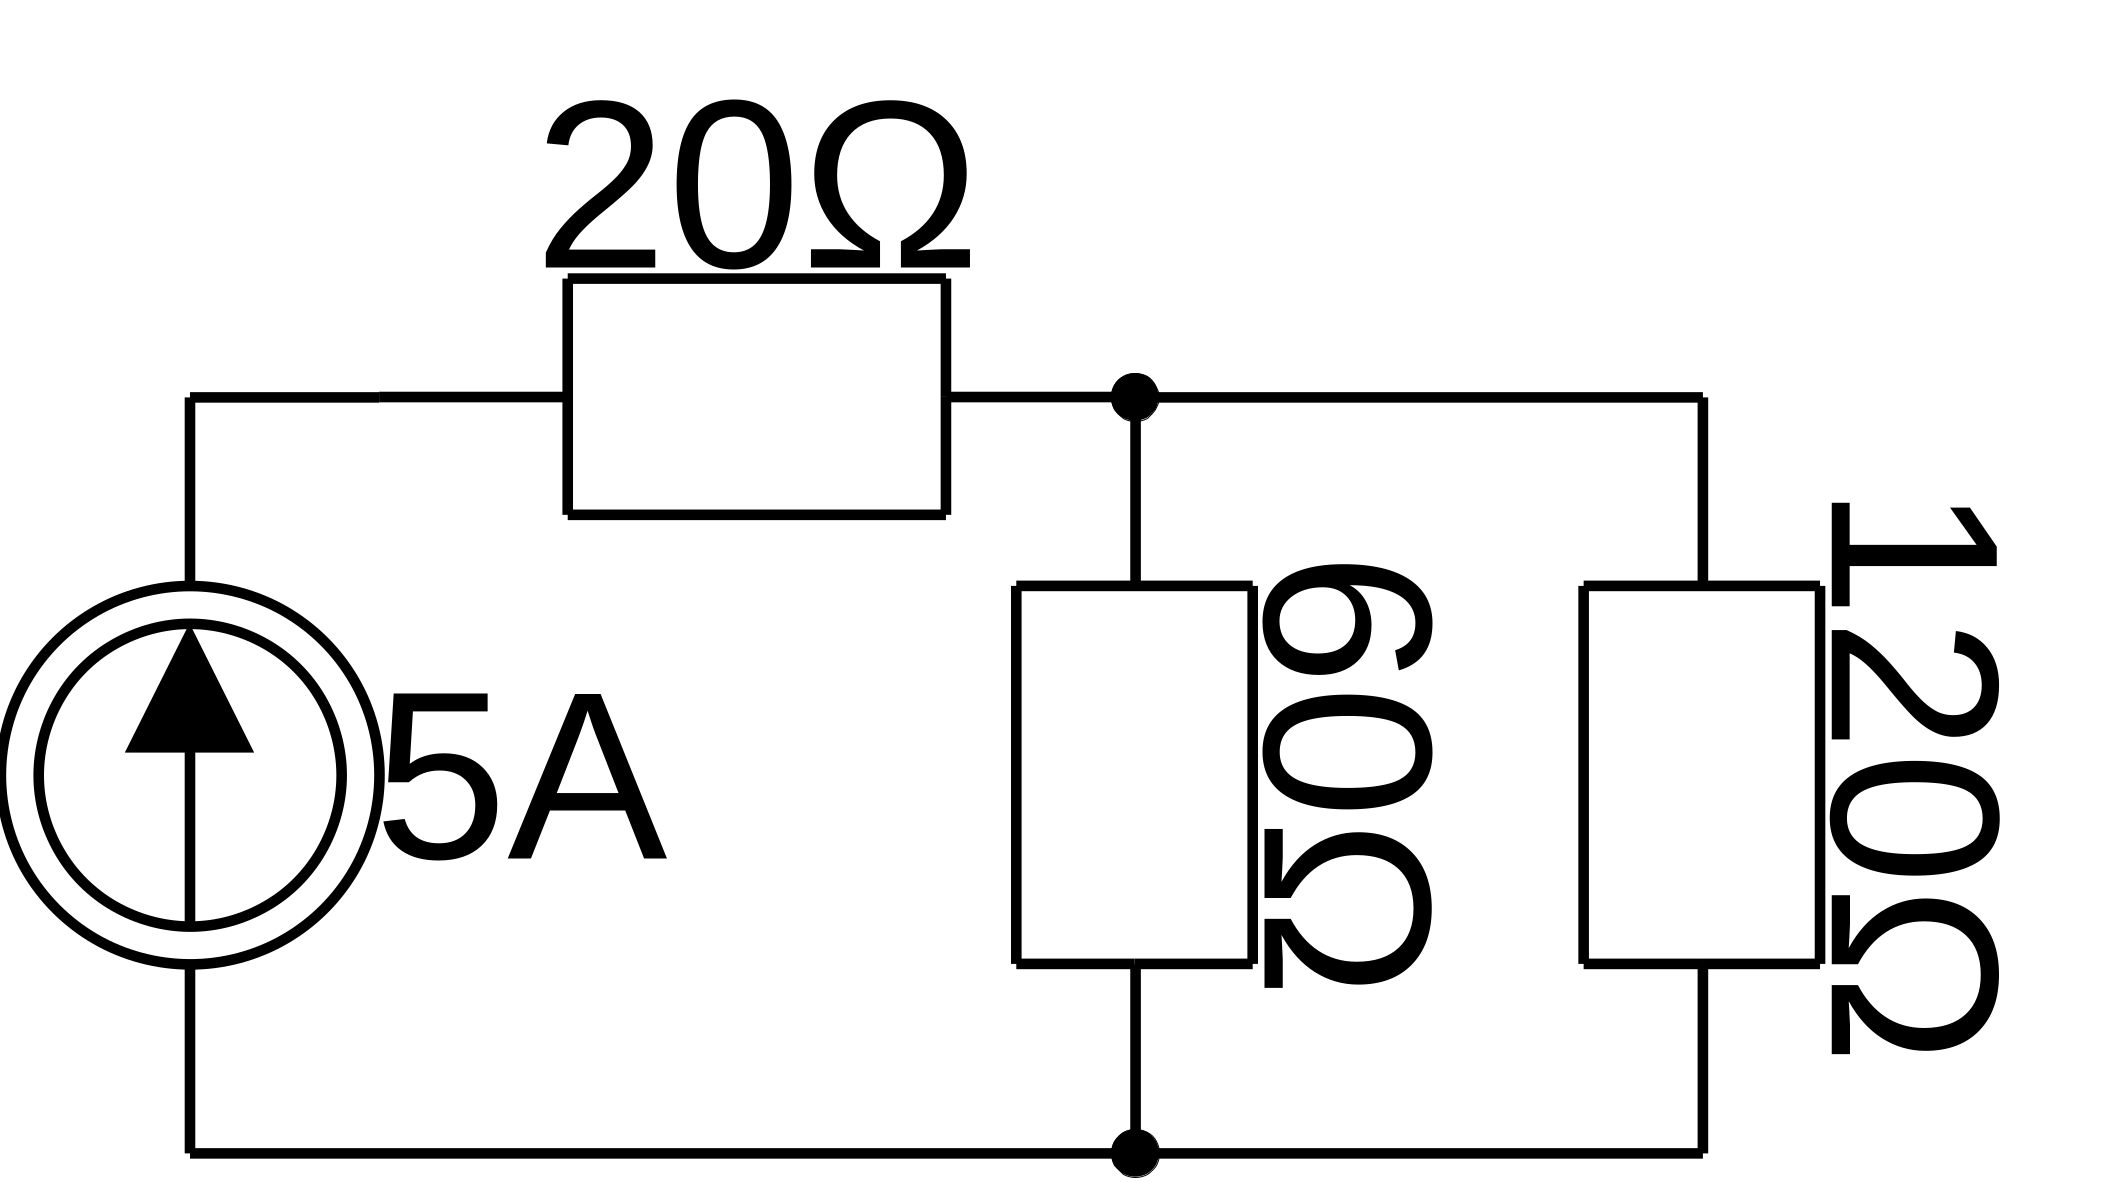
\includegraphics[scale=0.12, alt={}]{./imags/E02/2d.png}
		\caption{Zadanie 4. Oblicz wszystkie napięcia i prądy.}
	\end{figure}	
\end{frame}

\begin{frame}{Zadanie 5}
	\begin{figure}
		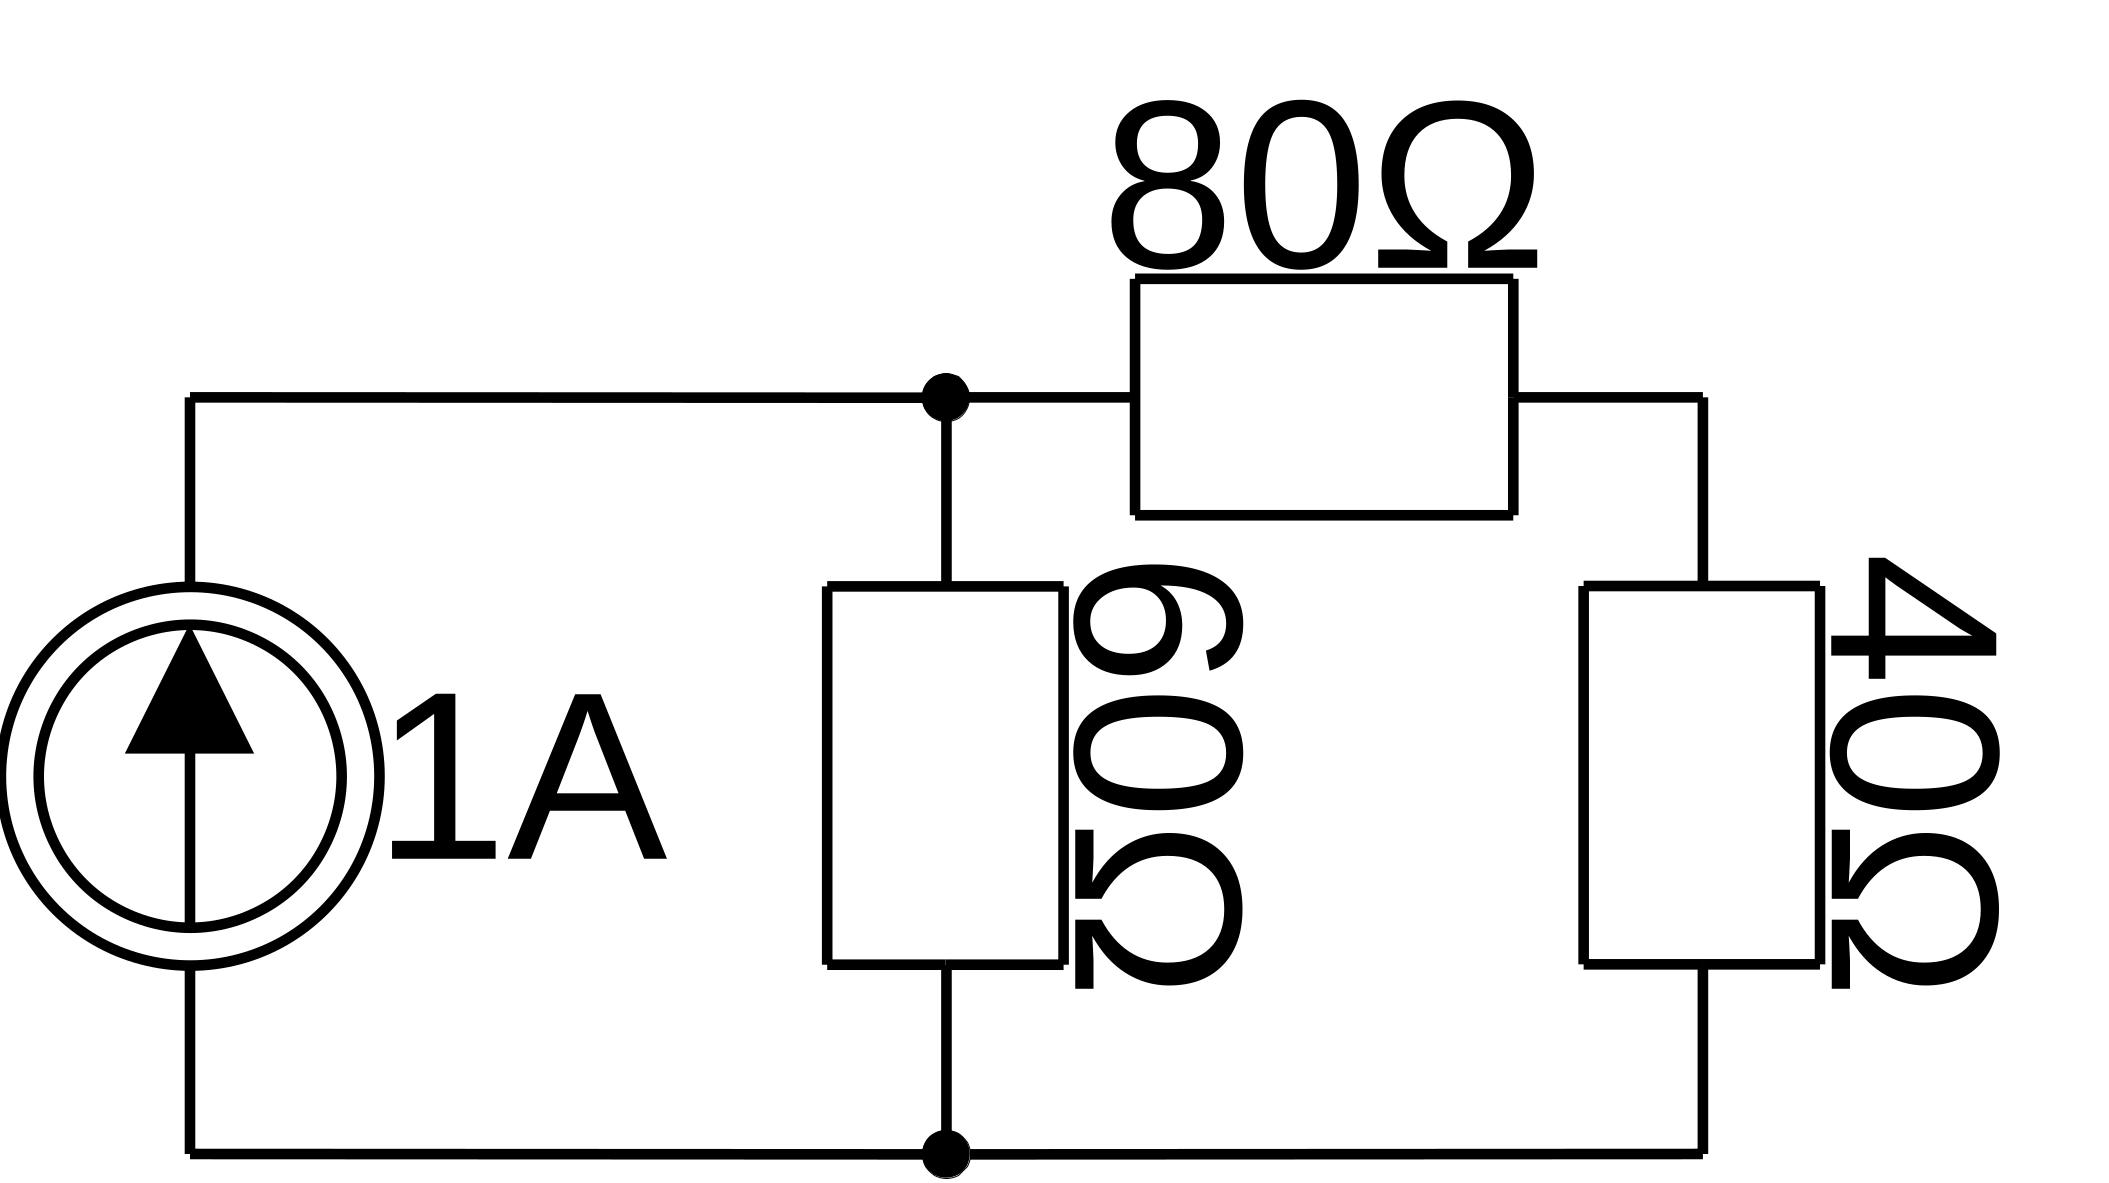
\includegraphics[scale=0.12, alt={}]{./imags/E02/2e.png}
		\caption{Zadanie 5. Oblicz wszystkie napięcia i prądy.}
	\end{figure}	
\end{frame}

\begin{frame}{Zadanie 6}
	\begin{figure}
		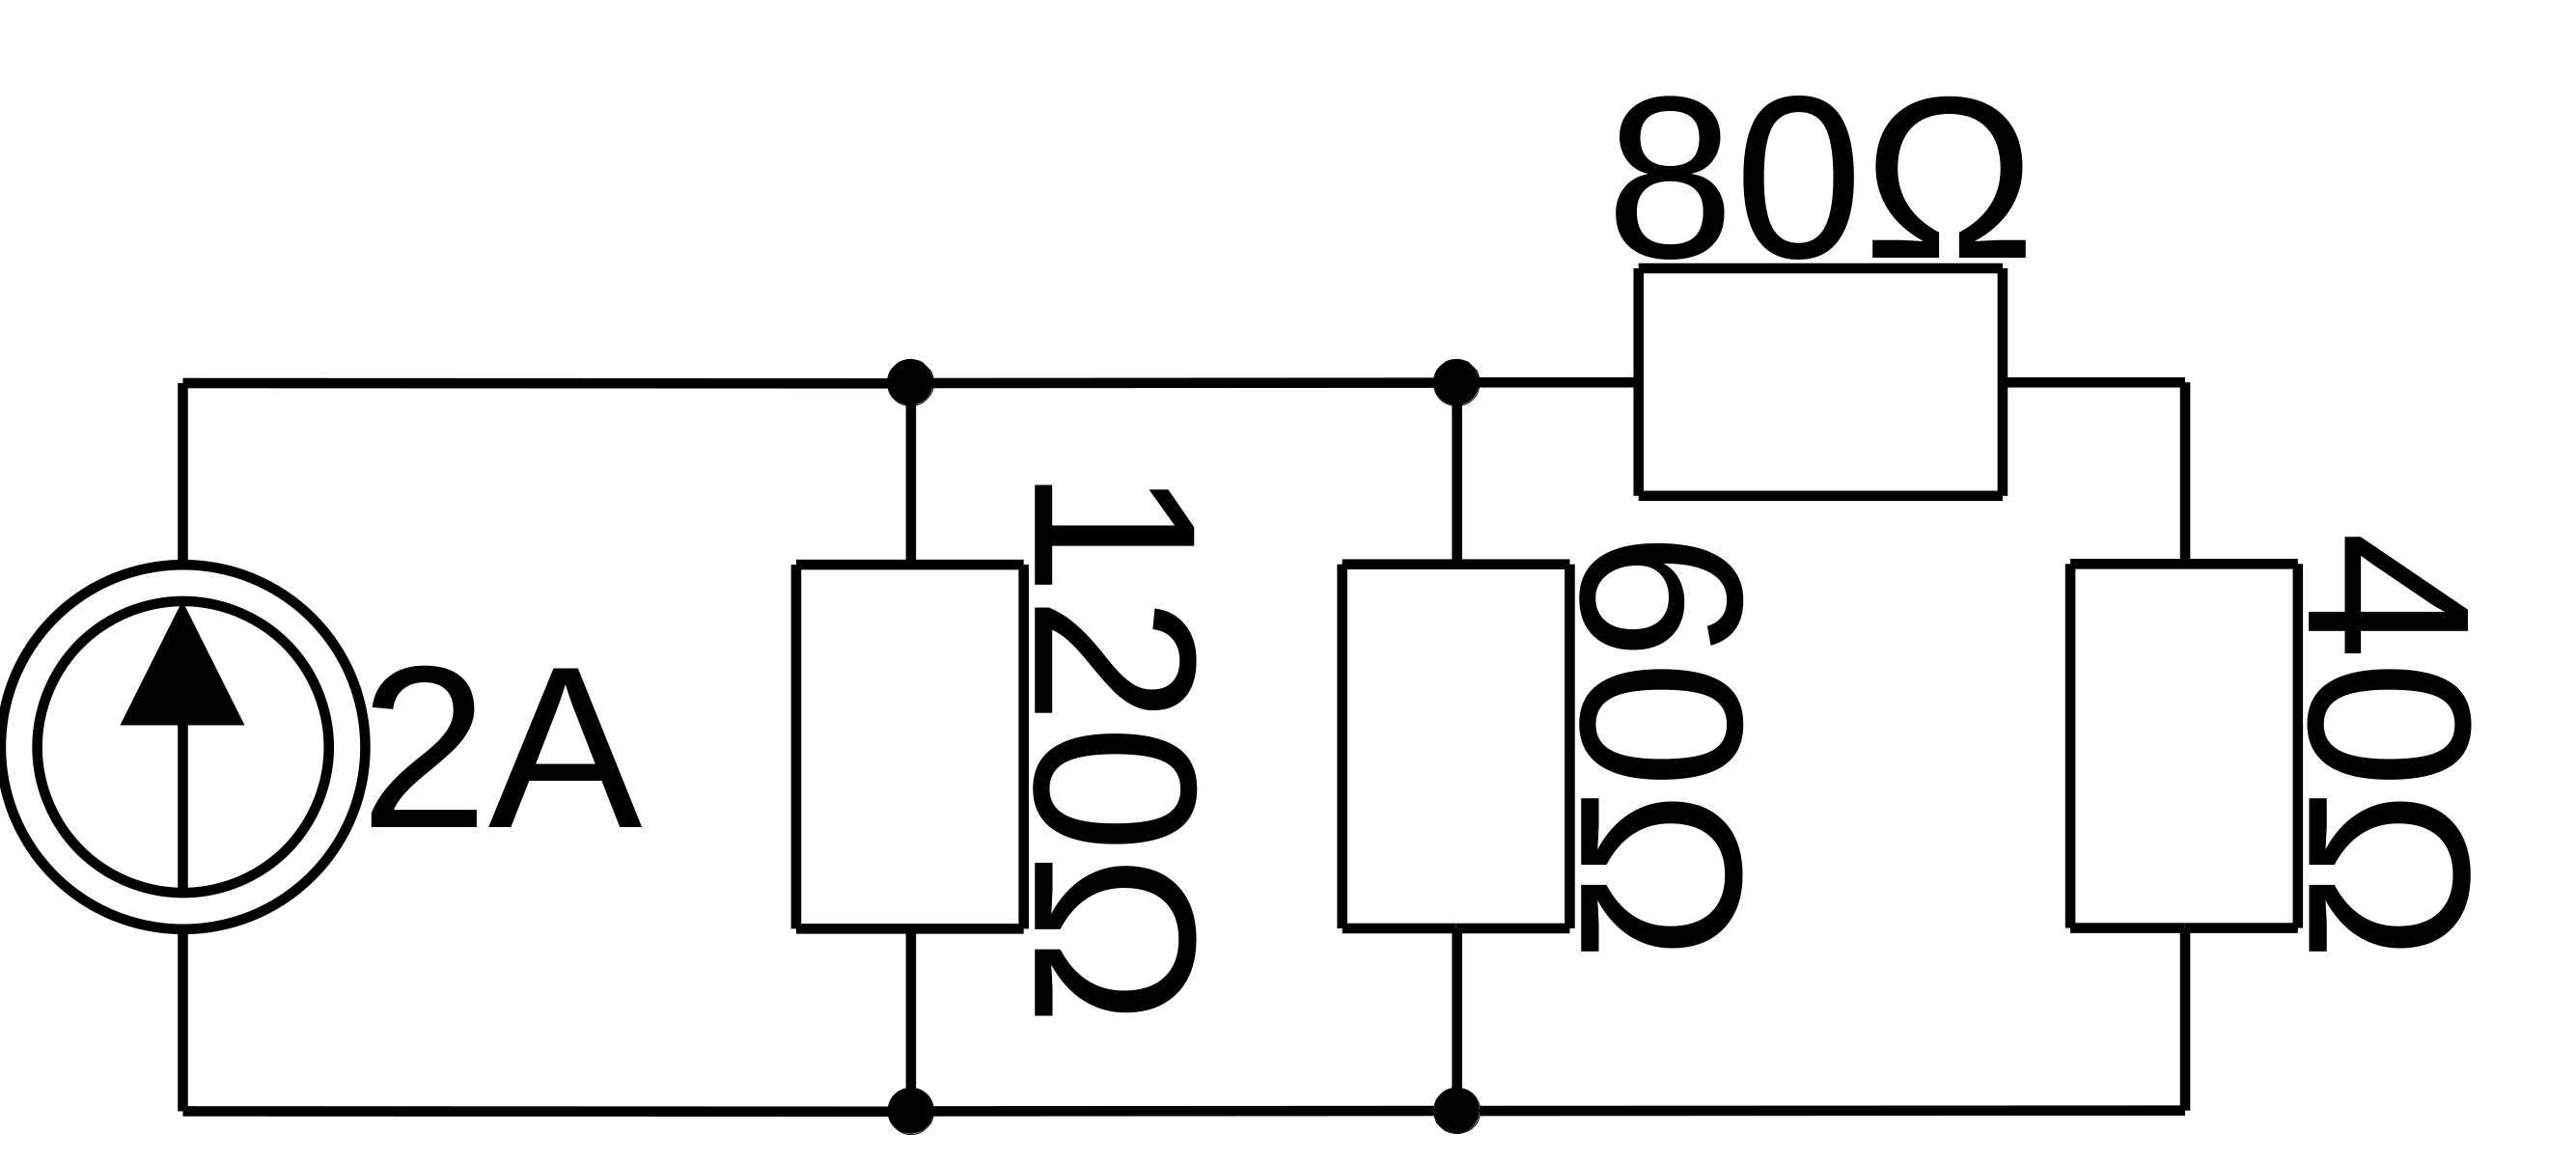
\includegraphics[scale=0.12, alt={}]{./imags/E02/2f.png}
		\caption{Zadanie 6. Oblicz wszystkie napięcia i prądy.}
	\end{figure}	
\end{frame}

\begin{frame}{Zadanie 7}
	\begin{figure}
		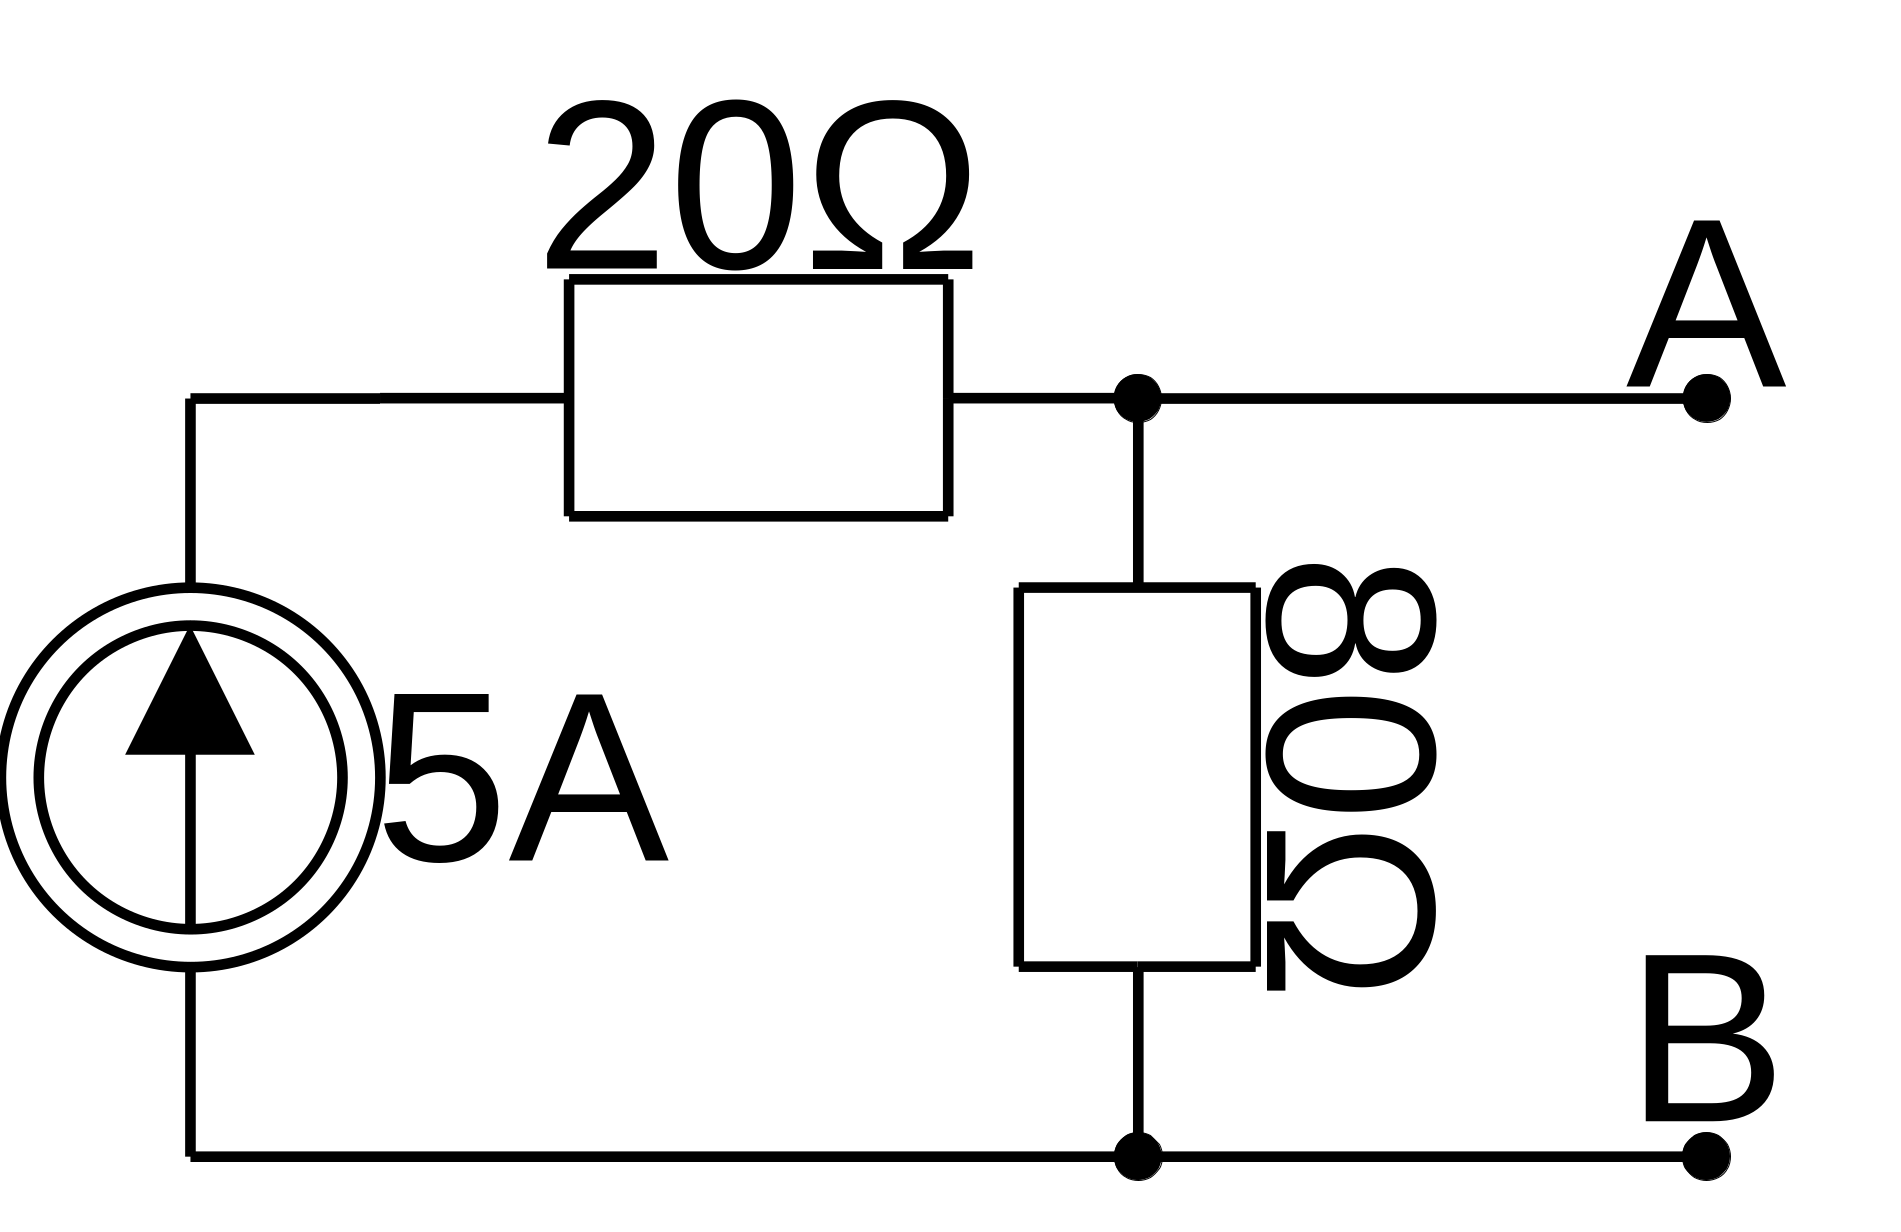
\includegraphics[scale=0.12, alt={}]{./imags/E02/2g.png}
		\caption{Zadanie 7. Znajdź zastępcze źródła Thevenina i Nortona z perspektywy wyprowadzeń A i B.}
	\end{figure}	
\end{frame}

\begin{frame}{Zadanie 8}
	\begin{figure}
		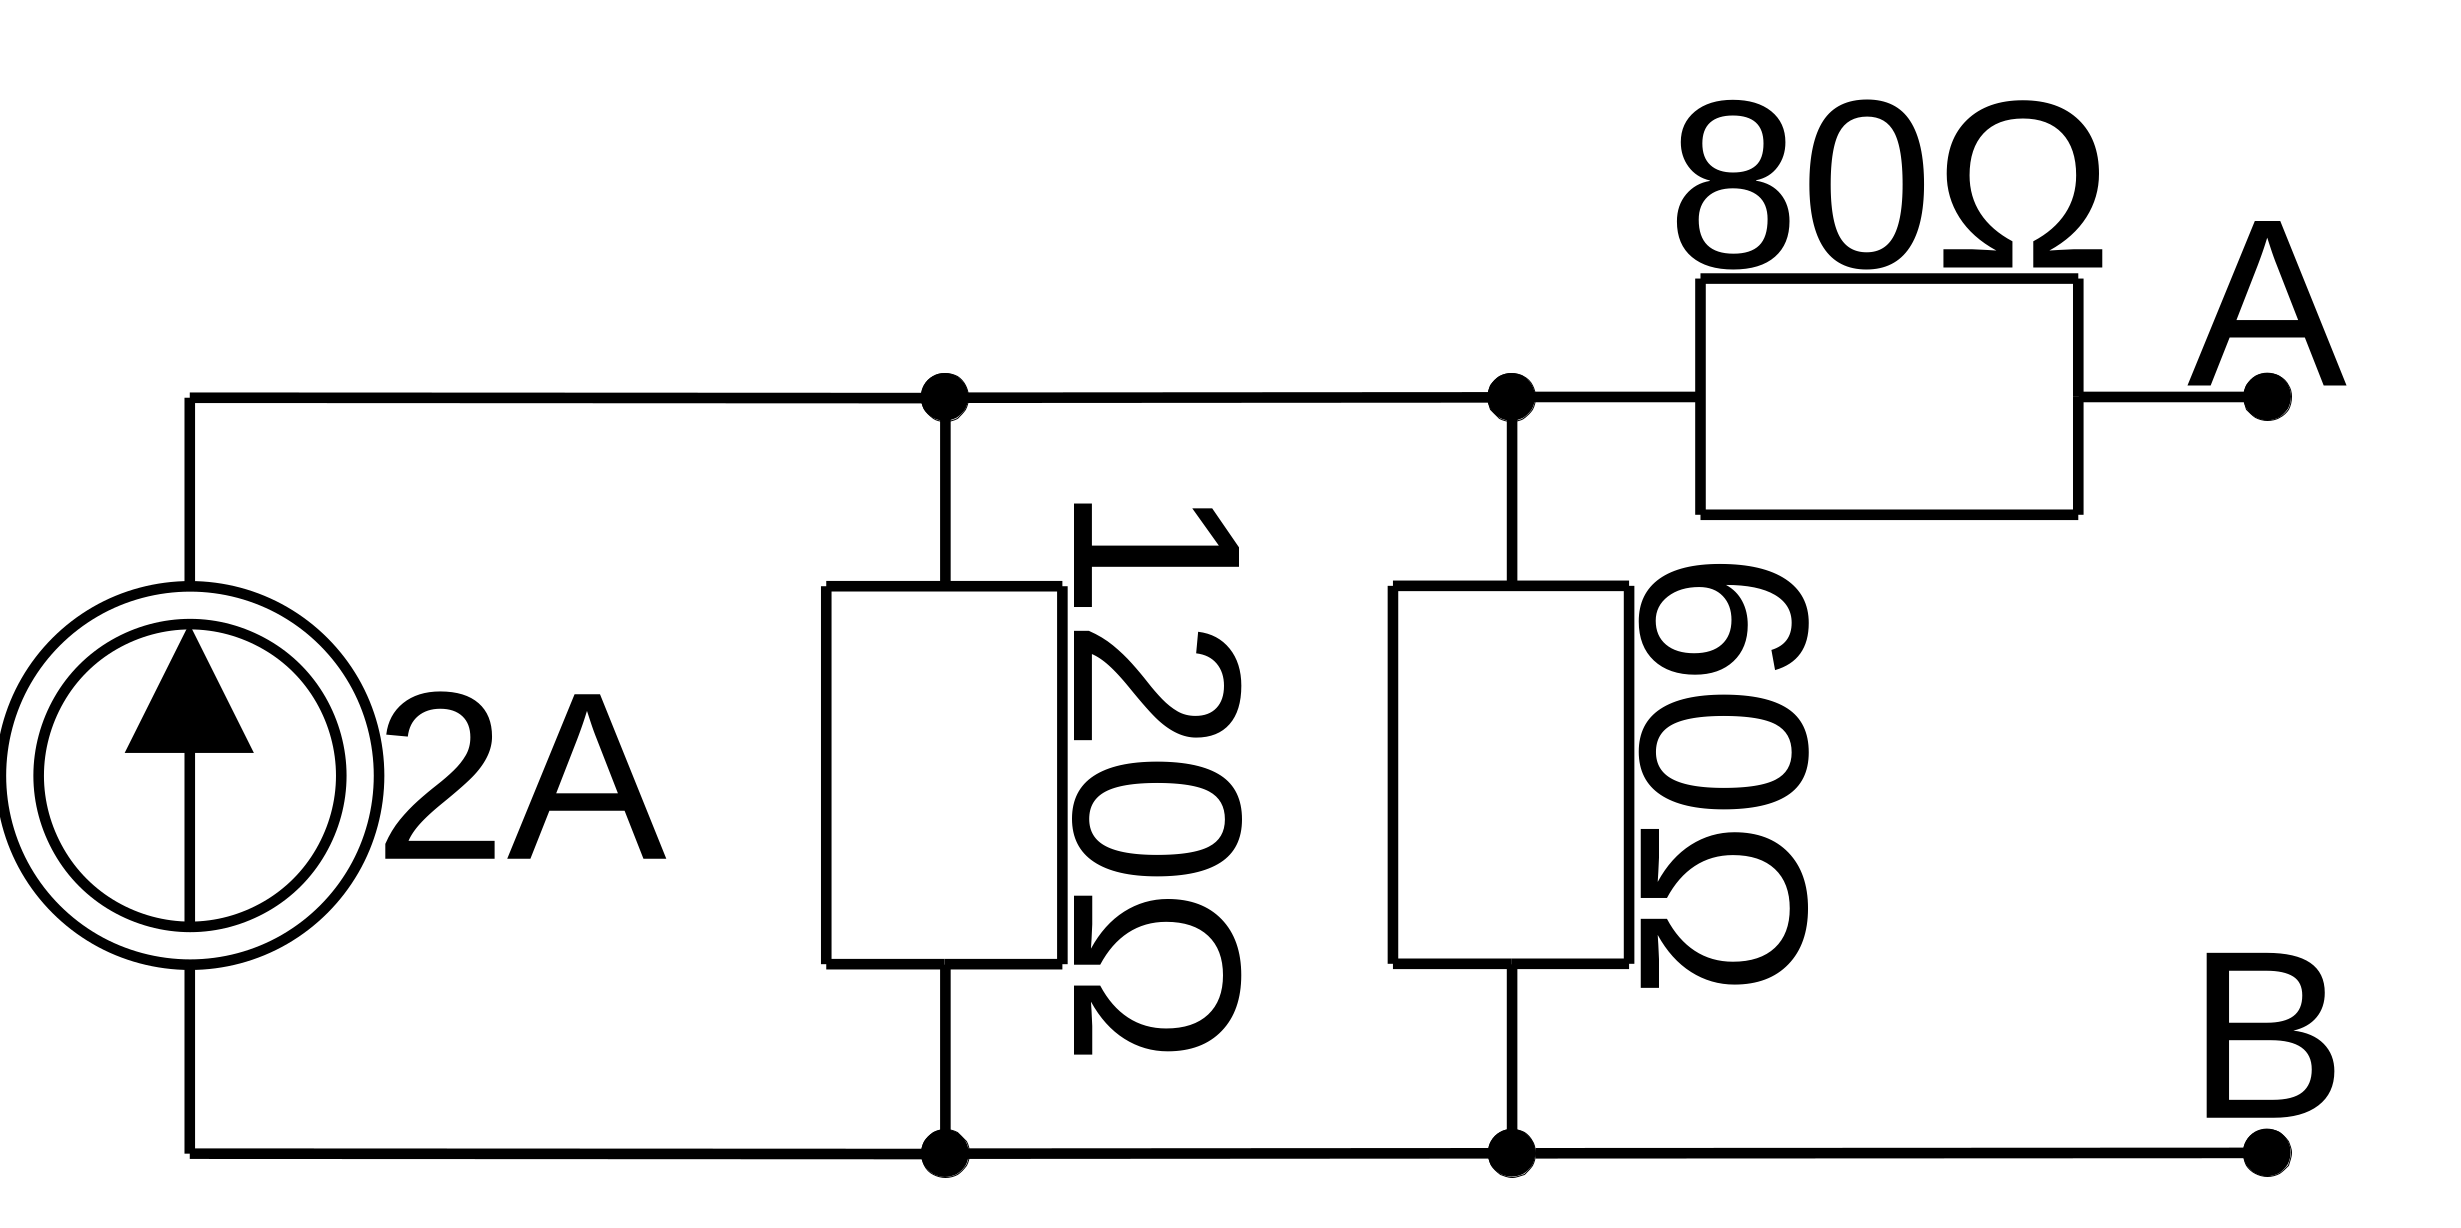
\includegraphics[scale=0.12, alt={}]{./imags/E02/2h.png}
		\caption{Zadanie 8. Znajdź zastępcze źródła Thevenina i Nortona z perspektywy wyprowadzeń A i B.}
	\end{figure}	
\end{frame}

\begin{frame}{Zadanie 9}
	\begin{figure}
		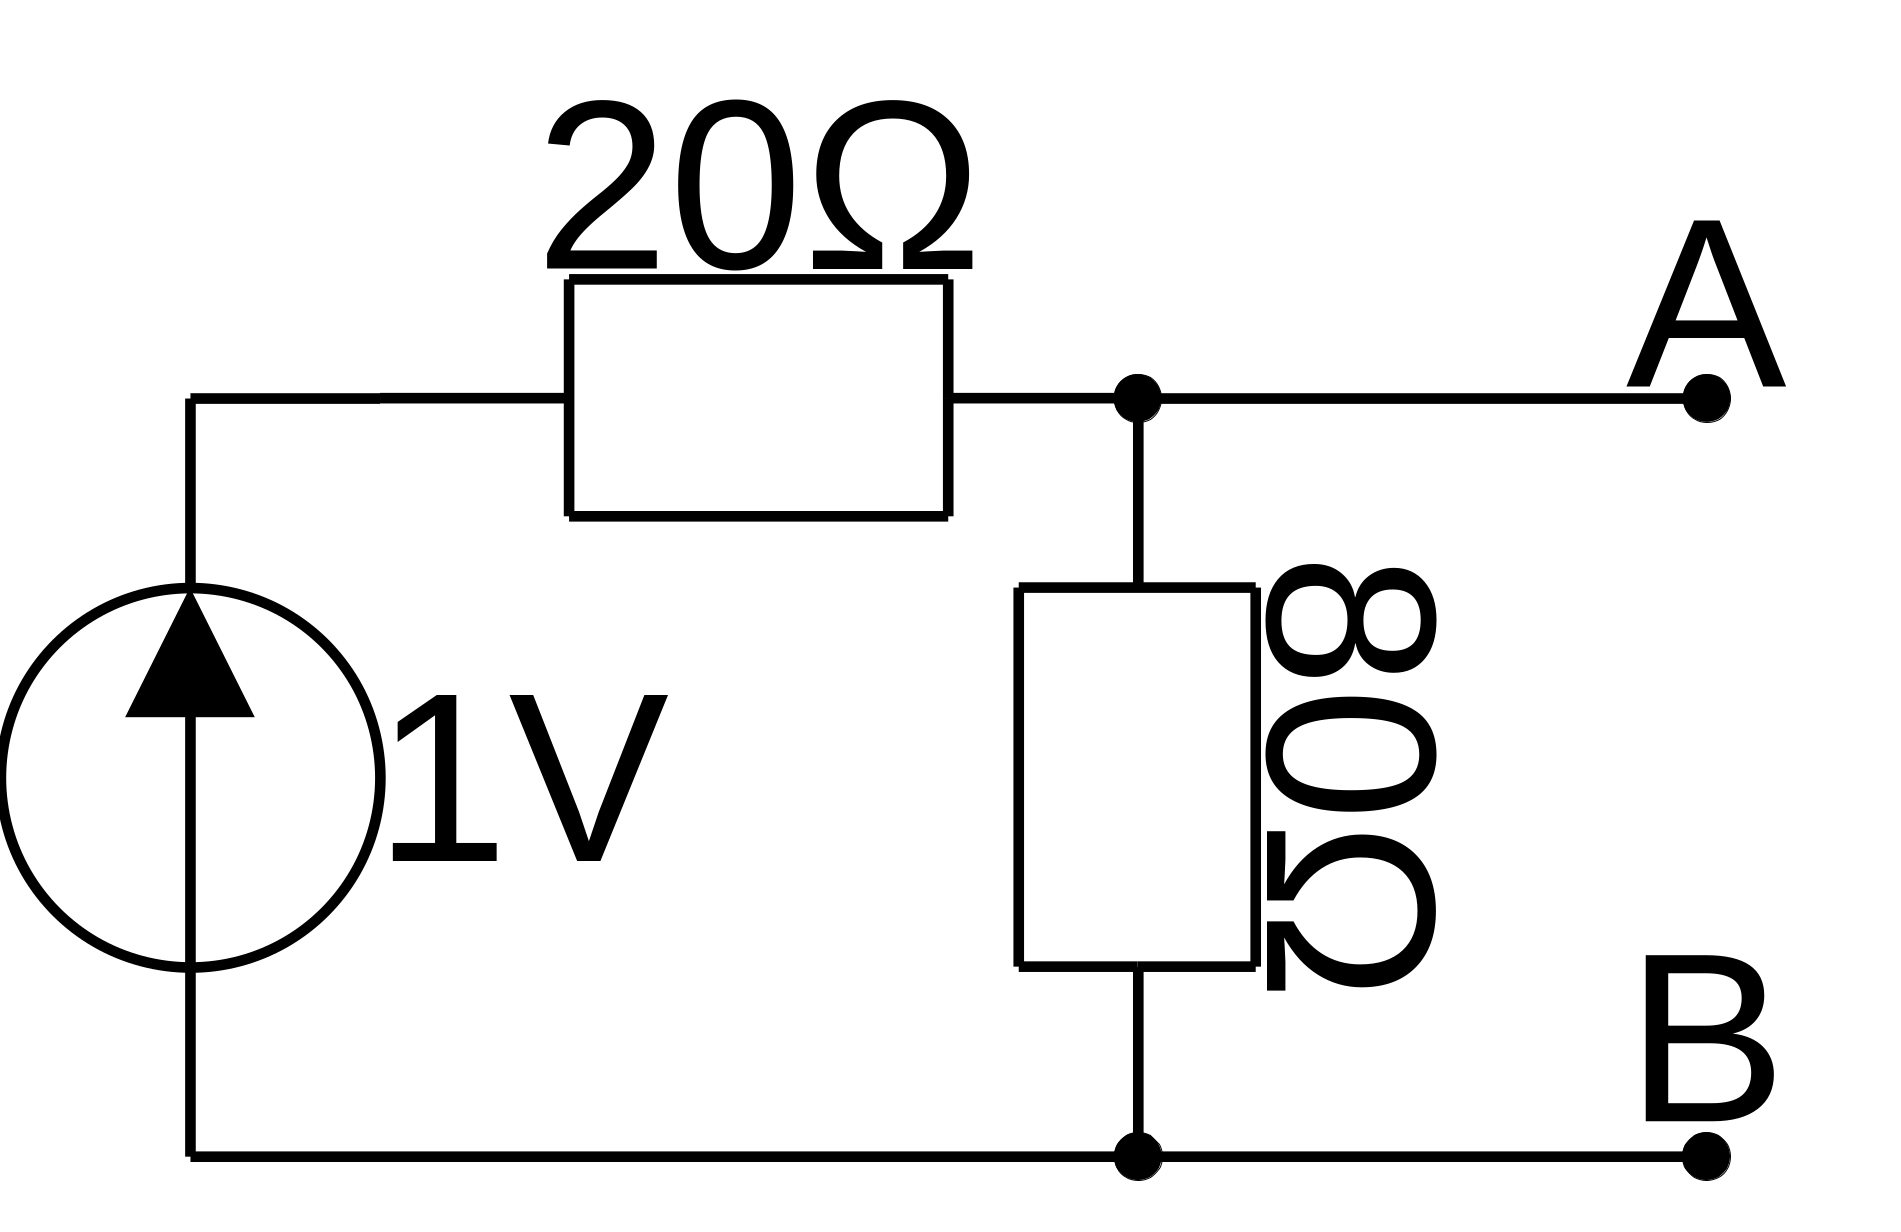
\includegraphics[scale=0.12, alt={}]{./imags/E02/2i.png}
		\caption{Zadanie 9. Znajdź zastępcze źródła Thevenina i Nortona z perspektywy wyprowadzeń A i B.}
	\end{figure}	
\end{frame}

\begin{frame}{Zadanie 10}
	\begin{figure}
		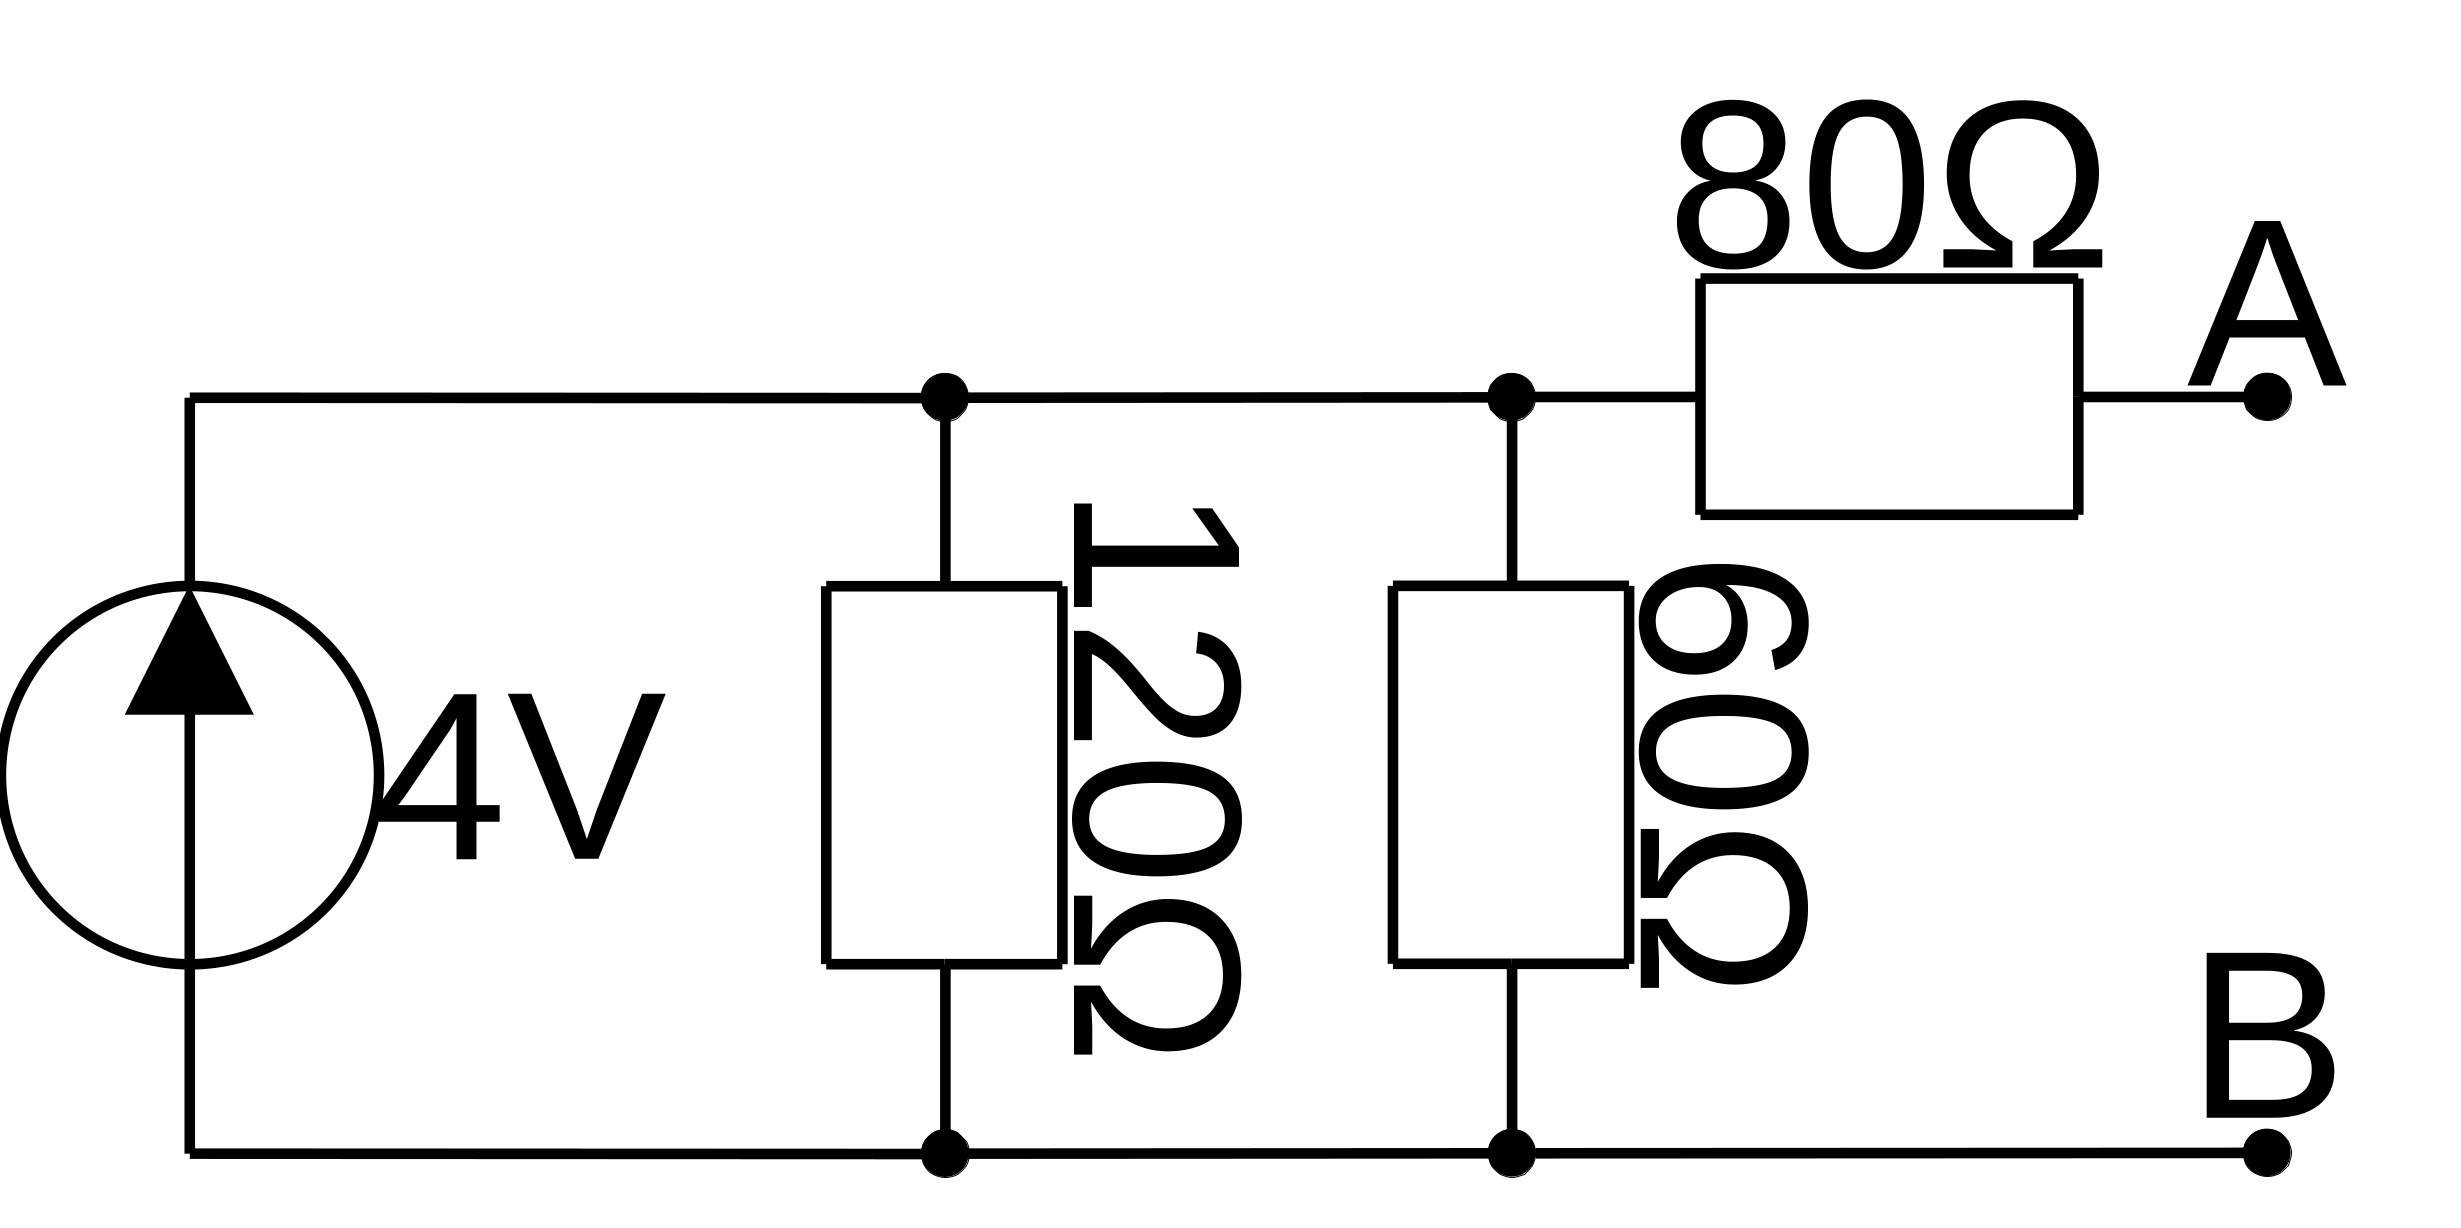
\includegraphics[scale=0.12, alt={}]{./imags/E02/2j.png}
		\caption{Zadanie 10. Znajdź zastępcze źródła Thevenina i Nortona z perspektywy wyprowadzeń A i B.}
	\end{figure}	
\end{frame}

\begin{frame}{Zadanie 11}
	\begin{figure}
		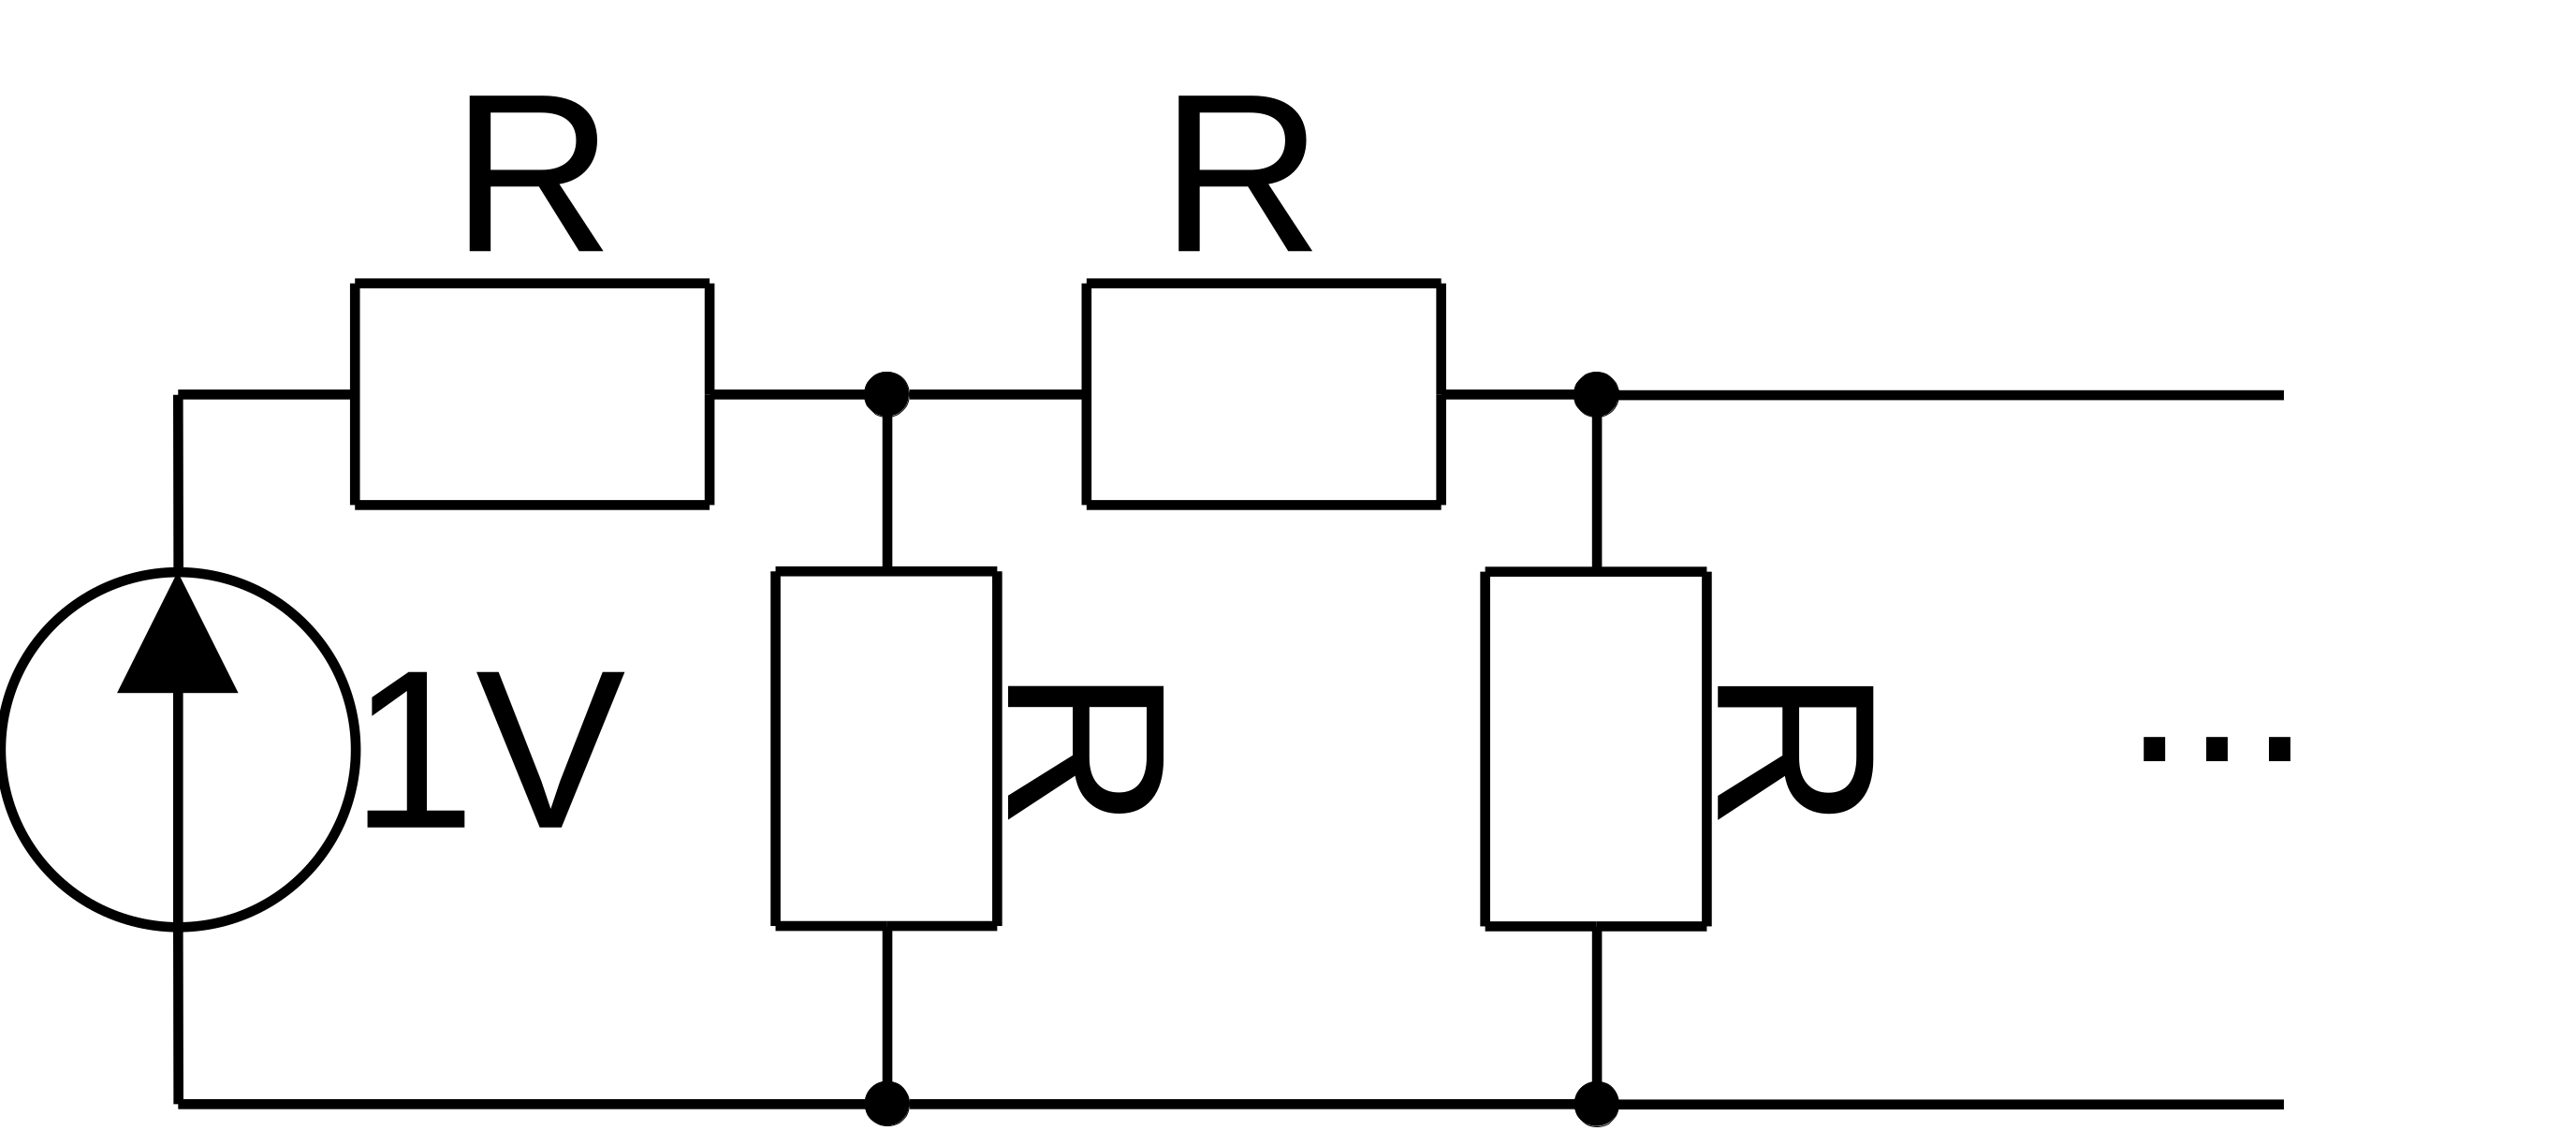
\includegraphics[scale=0.12, alt={}]{./imags/E02/2k.png}
		\caption{Zadanie 11. Znajdź prąd pobierany z źródła napięciowe.}
	\end{figure}	
\end{frame}

\begin{frame}{Zadanie 12}
	\begin{figure}
		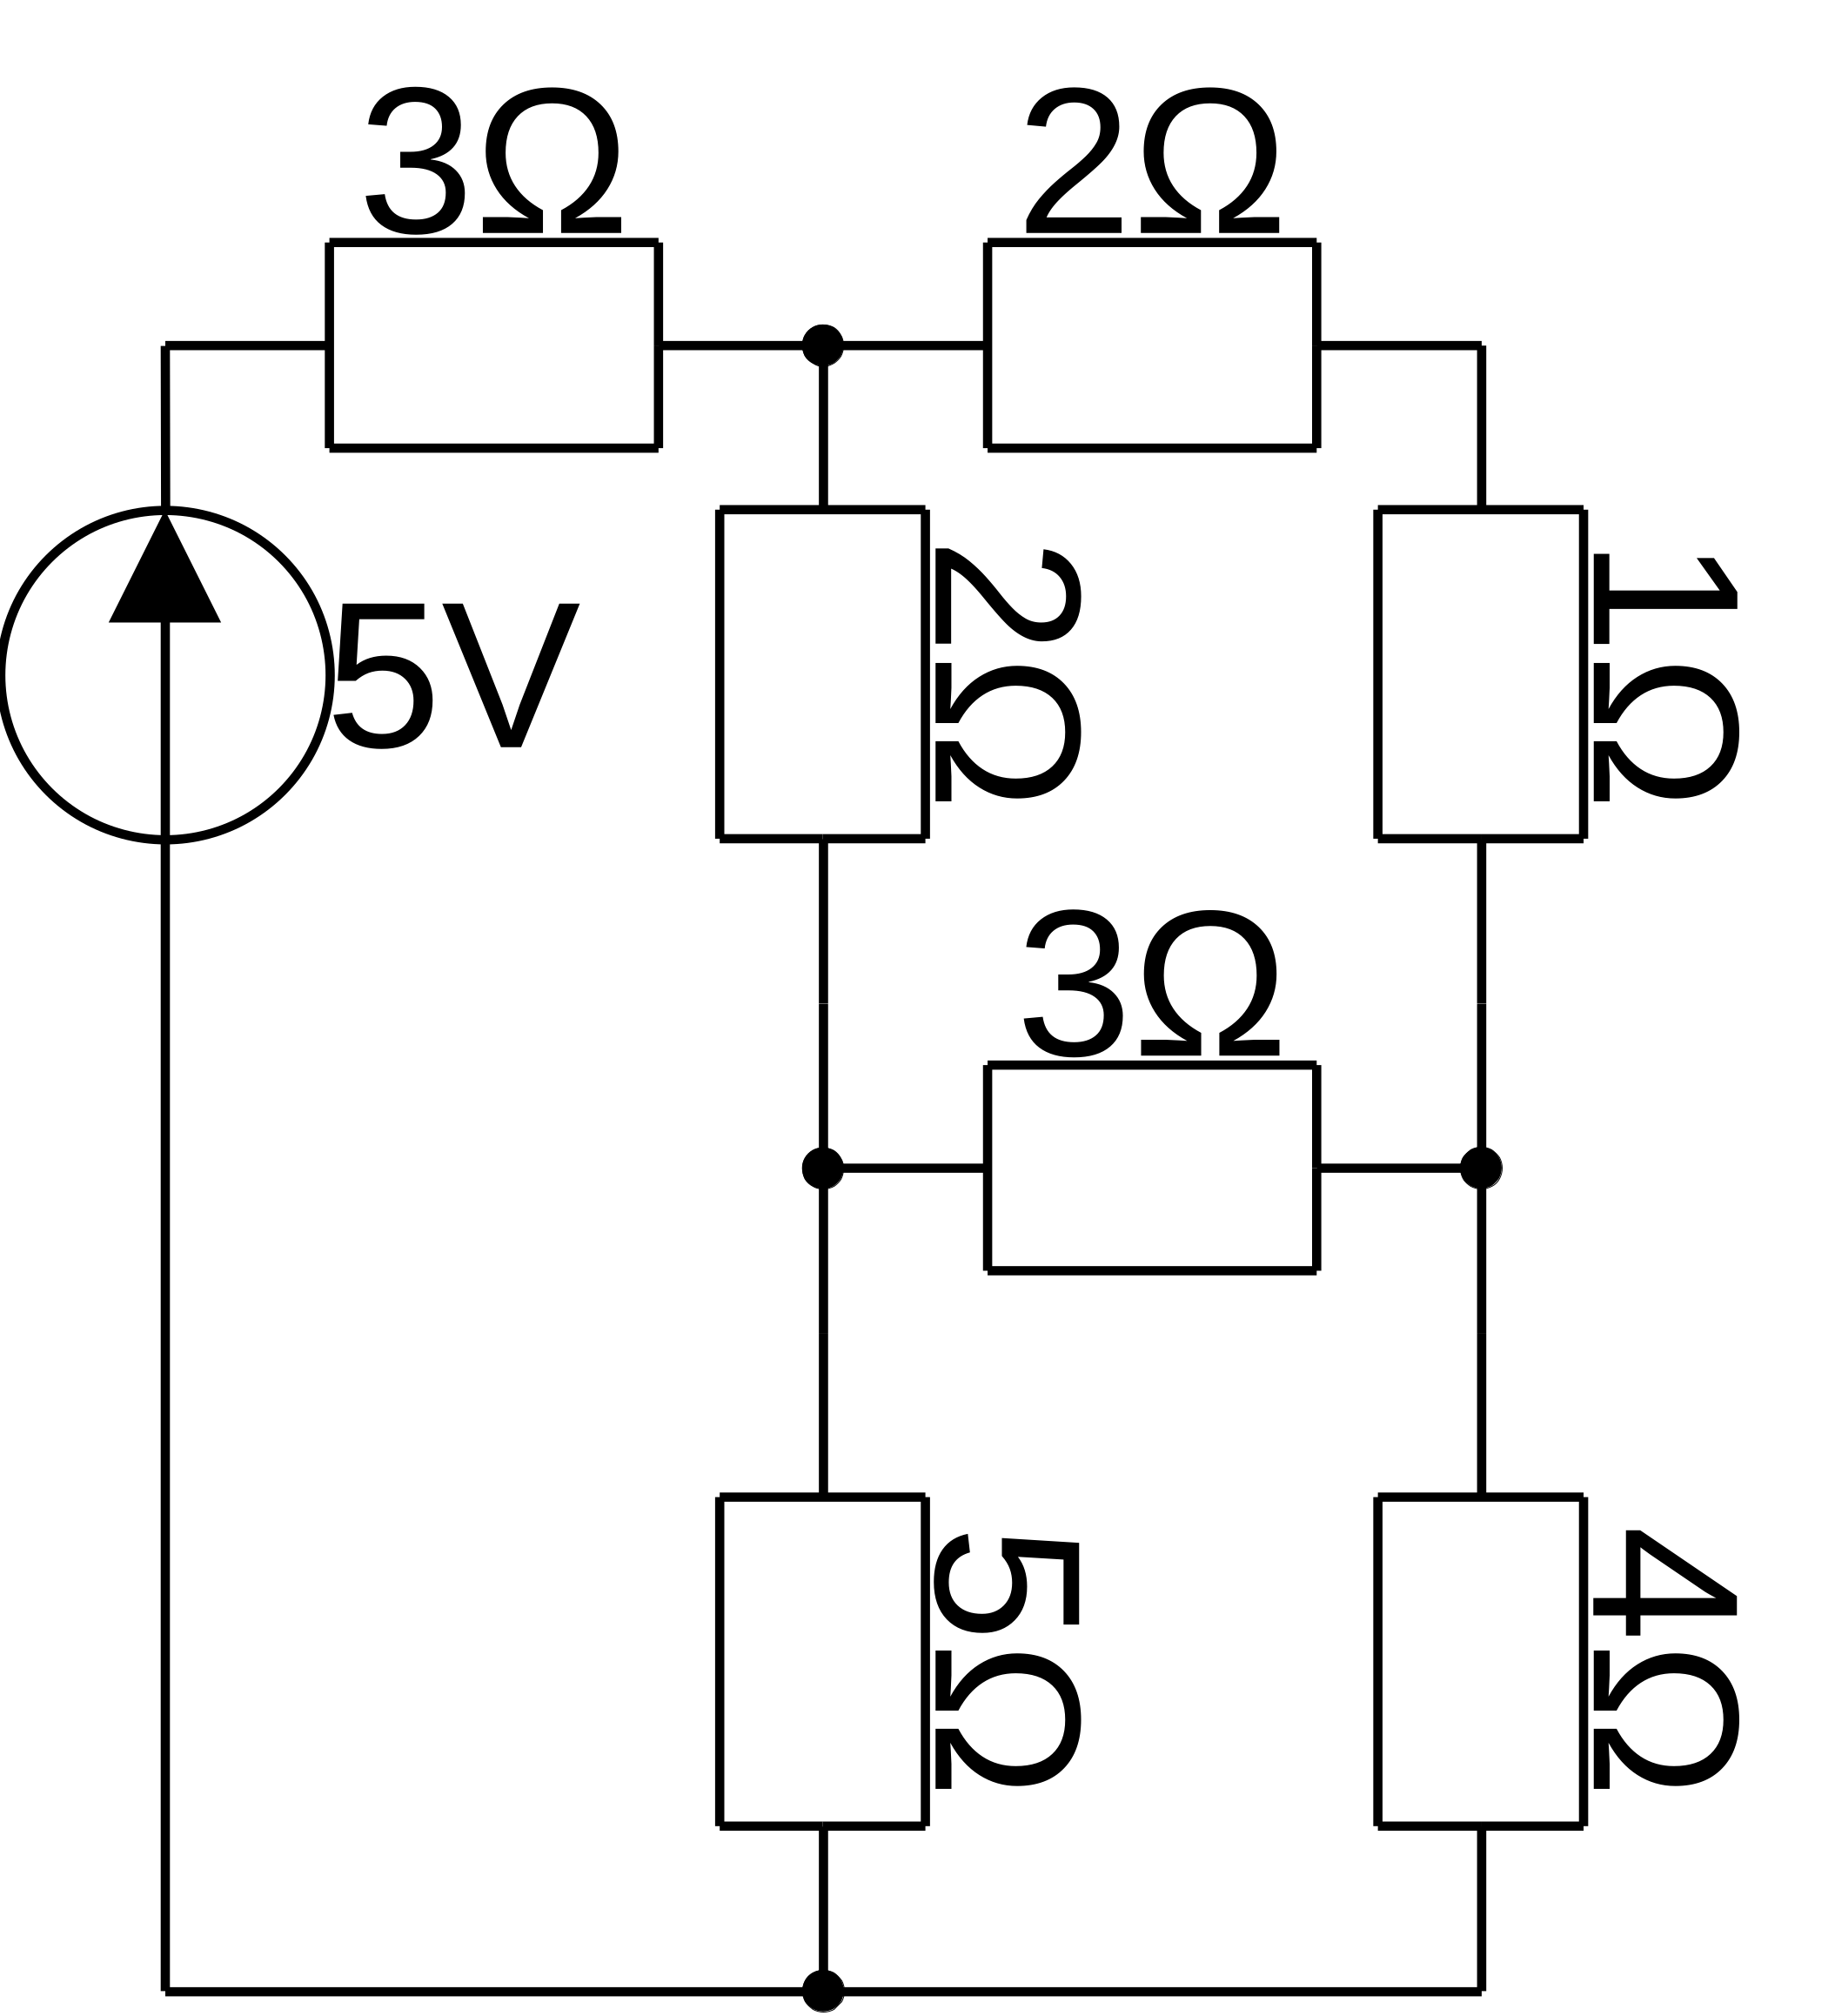
\includegraphics[scale=0.08, alt={}]{./imags/E02/2l.png}
		\caption{Zadanie 12. Wykonaj bilans mocy.}
	\end{figure}	
\end{frame}